\section{Patterns of Parallelism}\label{ch4}
In general, there exist some frequent \textbf{patterns of parallelism}, but we may need to design something quite specific for our problem/algorithm. We might identify two main techniques:

\begin{itemize}
    \item \textbf{decomposition techniques} (like \textit{divide-and-conquer}) that are used to generate (possibly) \textbf{independent sub-problems} that can be run in \textbf{parallel}. Notice that usually this is not a simple task, and also the merging phase of the outputs could be a problem;
    \item \textbf{mapping techniques} to decide who is going to execute what. These techniques depend on the \textbf{dependencies} among the tasks to be performed and their goal is to \textbf{maximize the load balance}.
\end{itemize}

\subsection{Task dependency graph (TDG)}
In general, the decomposition can be modelled with a \textbf{Task Dependency Graph} or \textbf{TDG}, which is a direct acyclic graph (DAG) where each \textbf{node} corresponds to a \textbf{task}, the \textbf{edges} represent task/data \textbf{dependencies} and the labels on the nodes measure the task computational cost.

\begin{figure}[h!]
		\centering
		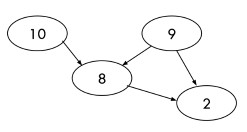
\includegraphics[scale = 2.0]{img/tdg.jpg}
        \label{tdg}
        \caption{Example of TDG}
\end{figure}

In this sense, the TDG is used to show the relationships between the tasks resulting from a decomposition, and is not unique for a given problem: each problem could have different decompositions, task size etc.., i.e. the TDG depends on the specific decomposition of the problem. Moreover, TDG can be used for discovering load balance and the order of execution of the tasks.

Now, we define \textbf{parallelism degree} the number of tasks that can be executed in parallel. Notice that this number may change during the execution of an application, but in general it increases with a fine-grained decomposition. Obviously, our goal is to obtain an high parallelism degree, in order to better exploit threads and parallel computations.

A \textbf{directed path in a TDG} is a sequence of tasks in the TDG (which cannot be executed in parallel) linked by a dependency relation. The length of the path is given by the sum of the weights (i.e. labels) of its nodes.

A \textbf{critical path} is the longest directed path in the TDG, and it represents the \textbf{bottleneck} of the application. In this sense, in represents the minimum execution time, i.e. $\text{total running time} \geq \text{critical path}$.

Finally, the \textbf{average parallelism degree} is defined as $\frac{\text{Total work}}{\text{Length of the critical path}}$, where Total work represents the sum of all the labels of the graph. This measure provides an estimation of how much work we can run in parallel, so the larger the result, the more work we can run in parallel. Our goal is to define a TDG with the shortest possible critical path, in order to maximize the work that can be done in parallel.

\subsection{Task interaction graph (TIG)}
In this case, the nodes represent the tasks, the edges represent interaction/data exchange, the node labels represent the computational cost and the edge labels represent the amount of data that is exchanged.

\begin{figure}[h!]
		\centering
		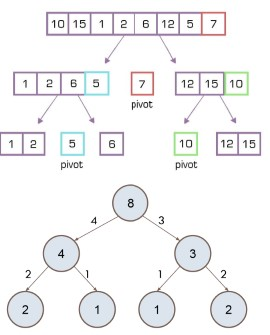
\includegraphics[scale = 2.0]{img/tig.jpg}
        \label{tig}
        \caption{Example of TIG}
\end{figure}

Our goal is to find the minimum cut (i.e. the cut with minimum weight) s.t. each partition has the same load.

\subsection{Mapping}
In general, the number of tasks exceeds the number of processors, so we have a \textbf{mapping problem}, i.e. we have to assign the tasks to the processors. Usually, this mapping is planned on the basis of TDG and TIG:

\begin{itemize}
    \item TDG helps in achieving load balance and minimizing waiting times (each processor receives the same load);
    \item TIG minimizes the interactions/communications between tasks (useful in a distributed environment).
\end{itemize}

Clearly, there can be a conflict between these two goals, but in general the \textbf{guidelines} are the following:

\begin{itemize}
    \item Assign independent tasks to different processors;
    \item Tasks on the critical path must be assigned as early as possible;
    \item Minimize the interaction/communication costs by scheduling "dense" sub-graphs of the TIG to the same processor.
\end{itemize}

We will now focus on some common patterns of parallelism:
\begin{itemize}
    \item Pipeline;
    \item Single Program Multiple Data / Data Parallel;
    \item Task Pool;
    \item Dynamic Task Creation.
\end{itemize}

\subsubsection{Pipeline}
A \textbf{pipeline} is a special kind of task-parallelism, where the \textbf{computation} is \textbf{partitioned} into stages that are executed sequentially: the output of a stage provides the input of the following one. 

\begin{figure}[h!]
		\centering
		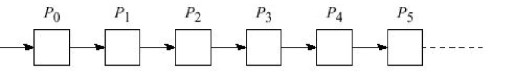
\includegraphics[scale = 2.0]{img/pipeline1.jpg}
        \label{pipeline1}
        \caption{Pipeline}
\end{figure}

\textbf{Asymptotically}, a pipeline achieves a speed-up equal to the number of stages. If we have $p$ processors, an input stream of $n$ elements and a cost of each task of $t$, then:

\begin{itemize}
    \item $(p-1)$ steps are used to fill the pipeline, in $(p-1)t$ time;
    \item $n$ steps are used to produce the output, in $nt$ time (each stage of the pipeline must be processed);
    \item The total speedup is $\frac{\text{sequential time}}{\text{parallel time}} = \frac{ptn}{nt + (p-1)t} = \frac{p}{1 + \frac{p-1}{n}} \rightarrow p$
\end{itemize}

In this sense, if each stage has the same load of work, then we reach a \textbf{linear speedup}.

\begin{figure}[h!]
		\centering
		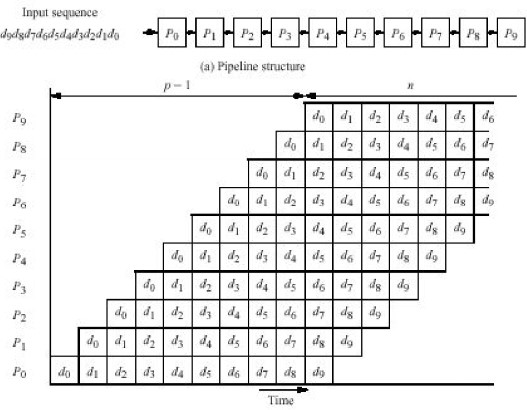
\includegraphics[scale = 2.0]{img/pipeline2.jpg}
        \label{pipeline2}
        \caption{Execution of a pipeline}
\end{figure}

\subsubsection{Single Program Multiple Data}
This strategy addresses to problems that can be solved with a large set of completely independent sub-tasks, i.e. in case of a completely disconnected TDG. Clearly, this is not a common scenario, but for example involves the Mandelbrot problem.

\begin{figure}[h!]
		\centering
		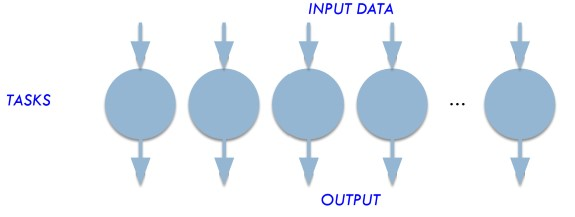
\includegraphics[scale = 1.5]{img/SPMD.jpg}
        \label{spmd}
        \caption{Single Program Multiple Data}
\end{figure}

\subsubsection{Task Pool}
In this case the task list is stored in a shared data structure, we have a fixed number of threads and each thread dynamically picks a task and executes it. Clearly, this technique is characterized by a synchronization overhead, and a thread may possibly generate a new task too.

\begin{figure}[h!]
		\centering
		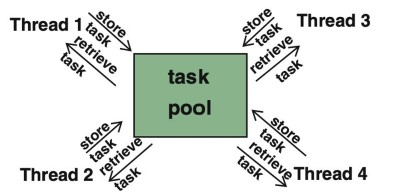
\includegraphics[scale = 1.7]{img/task pool.jpg}
        \label{task pool}
        \caption{Task Pool}
\end{figure}

In the Mandelbrot problem, there's a static partitioning of the input, assigning one pixel per task, then each thread processes a portion of the input, with dynamic assignment.

\subsubsection{Dynamic Task Creation}
In this technique, each thread can dynamically create new tasks, and it is useful to:

\begin{itemize}
    \item Improve the \textbf{parallelism degree};
    \item Adapt to task of unknown costs, since it can split a long task into smaller ones;
    \item Adapt to non uniform resources, since it can exploit multiple machines with different computing power.
\end{itemize}

Notice that a \textbf{task queue} must be shared among a pool of threads. This technique is very common, since it allows to deal with very different tasks.

\textbf{Distributed Load Balancing}

The goal of this approach is to remove centralization, i.e. remove the concept of \textit{master node}, and to favor data exchange among neighbors. There exist two different variant for this technique:

\begin{itemize}
    \item Push/Sender-Initiated, in which the worker that generates a new task sends it to another worker, instead of putting it in the task list;
    \item Pull/Receiver-Initiated, in which when a worker is idle, it asks other workers for a job to execute (work stealing)
\end{itemize}

\begin{figure}[h!]
		\centering
		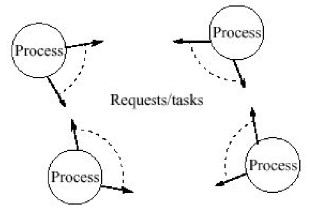
\includegraphics[scale = 2.0]{img/distributed load balancing.jpg}
        \label{distr load balancing}
        \caption{Distributed Load Balancing}
\end{figure}

In the Push/Sender-Initiated, the worker to which the task is sent can be selected:

\begin{itemize}
    \item At \textbf{random}, among all the workers;
    \item \textbf{Global Round Robin (GRR)} in which a global random variable/marker points to the "next" worker, and a worker needing a partner reads and increments the global variable;
    \item \textbf{Local Round Robin (LRR)}, in which each processor keeps a private pointer to the next available worker, so there's no overhead due to sharing a global variable.
\end{itemize}

In general, the choice among \textbf{static mapping} (pipeline, single program multiple data) and \textbf{dynamic mapping} (task pool, dynamic task creation) can be made according to the following schema:

\begin{figure}[h!]
		\centering
		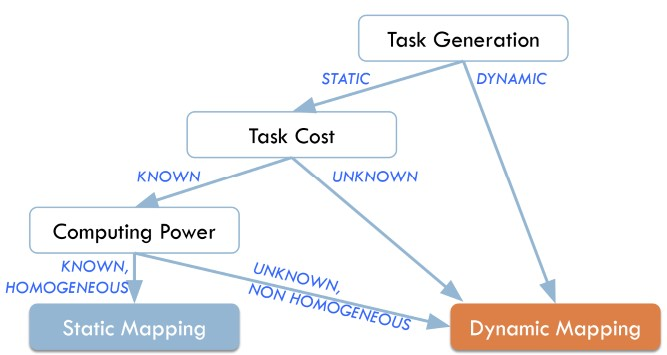
\includegraphics[scale = 1.8]{img/dynamic vs static mapping.jpg}
        \label{dy vs st}
        \caption{Static vs dynamic mapping}
\end{figure}

In general, the \textbf{static mapping} is preferable, since is does not need any synchronization.

\subsection{Prefix sum}
Given a list of integers $x_0, x_1, .., x_{n-1}$, compute the partial sum up to index $i$, for each $i$. 

The optimal sequential algorithm has complexity $O(n)$: for ($i$ = 1; $i<n$; $i++$) : $x[i] += x[i-1]$.

However, this algorithm is difficult to be parallelized, since each iteration depends on the previous one. For example, we cannot split the vector $x$ into two parts $T_1$ and $T_2$, since $T_2$ must wait $T_1$ to perform its computations. For this reason, the naive parallel algorithm works as follows:

\begin{itemize}
    \item Break the dependencies through a step-wise algorithm;
    \item One thread computes one element at each step.
\end{itemize}

\begin{figure}[h!]
		\centering
		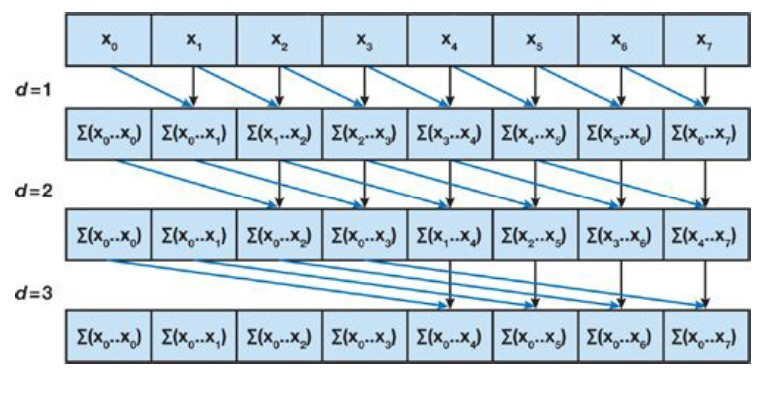
\includegraphics[scale = 1.6]{img/parallel prefix sum .jpg}
        \label{parallel prefix sum}
        \caption{Parallel prefix sum}
\end{figure}

In this case:

\begin{itemize}
    \item The total amount of work is $O(N \log N)$, where $\log N$ is the number of steps of the algorithm, and $N$ is the length of the vector. In the sequential version, the amount of work was $O(N)$;
    \item The complexity is $O(\log N)$, while in the sequential algorithm we had $O(N)$.
\end{itemize}

As we can see, in this case the parallel version of the algorithm is quite different from the sequential one, and we also notice that the parallel version results in more work to be done, but the execution time is faster. For this reason, in this case the benefits of the parallel algorithm can be obtained only if enough processors are available, otherwise it is better to execute the sequential algorithm.

\begin{figure}[h!]
		\centering
		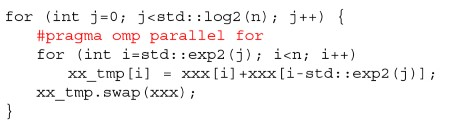
\includegraphics[scale = 1.6]{img/prefix sum algo.jpg}
        \label{prefix sum algo}
        \caption{Implementation of the parallel algorithm}
\end{figure}

For this reason, now our goal is to \textbf{reduce the amount of work}, i.e. number of sums, in order to reduce the number of processors that are needed for the parallelization.

The idea is to focus on an \textbf{exclusive prefix sum}, i.e. a prefix sum that discards the last element, which is composed on two phases: the \textbf{Up-sweep} phase and the \textbf{Down-sweep} phase. 

\begin{figure}[h!]
		\centering
		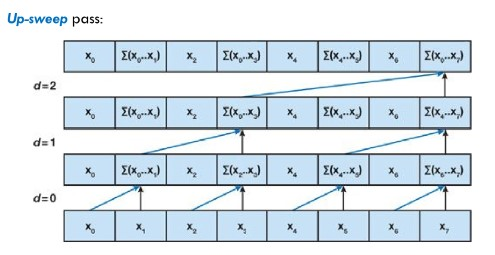
\includegraphics[scale = 2.0]{img/up-sweep.jpg}
        \label{up-sweep}
        \caption{Up-sweep phase}
\end{figure}

On the one hand, the goal of the \textbf{Up-sweep} phase is to store in a vector some important partial sums. In particular, it performs $N-1$ summations in $\log N$ steps, and the resulting vector contains several \textbf{correct partial sums}, together with elements for which the prefix sum is not computed. In this sense, an important property of the resulting vector is that each node that contains the correct partial sums holds the \textbf{sum of its children}.


\begin{figure}[h!]
		\centering
		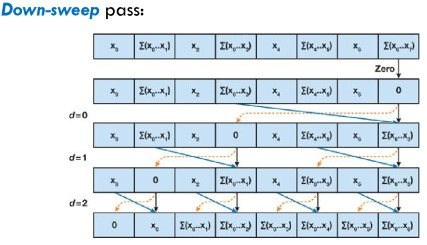
\includegraphics[scale = 2.0]{img/down-sweep2.jpg}
        \label{down-sweep}
        \caption{Down-sweep phase}
\end{figure}

On the other hand, the idea of the \textbf{Down-sweep} is to enforce the property that \textbf{each node should have the sum of all the leaves preceding it}, i.e. before its leftmost child. This means that:

\begin{itemize}
    \item The root has value 0;
    \item A \textbf{left} child has the same predecessors of its parent, so it has the \textbf{same value as it's parent};
    \item A \textbf{right} child is preceded by its parent predecessors plus the sibling's children, so its value should be equal to its \textbf{parent plus the up-sweep value of its sibling}.
\end{itemize}

This phase takes $\log N$ steps and $N-1$ summations, so the overall algorithm:

\begin{itemize}
    \item Has  complexity of $O(\log N)$ (i.e. number of steps);
    \item Performs $O(N)$ summations (amount of work), which is much less that the previous parallel version of the algorithm. Moreover, notice that a large parallelism degree can be exploited for most steps.
\end{itemize}

Picture \ref{gpu} shows the performances of the sequential algorithm (CPU), the naive parallel algorithm (Naive) and a version of the algorithm running on graphic processors (CUDA).

\begin{figure}[h!]
		\centering
		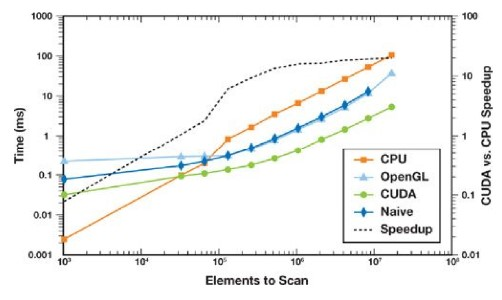
\includegraphics[scale = 1.5]{img/gpu perf.jpg}
        \label{gpu}
        \caption{GPU performance}
\end{figure}

\subsection{QuickSort}
We now focus on the problem of parallelizing the \textbf{QuickSort} algorithm.

\begin{figure}[h!]
		\centering
		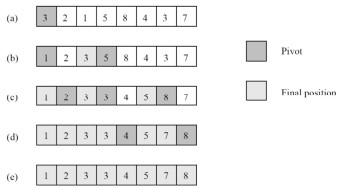
\includegraphics[scale = 2.0]{img/quicksort.jpg}
        \label{quicksort}
        \caption{QuickSort algorithm}
\end{figure}

A naive approach would be of running step (a) as 1 sequential task, step (b) as 2 parallel tasks, step (c) as 4 parallel tasks, and so on.., until the number of tasks is equal to available parallelism. However, this approach, and in general this algorithm, could lead to two important \textbf{issues}:


\begin{itemize}
    \item \textbf{Load imbalance}, since the pivot does not split the array in a balanced way, so the recursion in one side could complete the computation before the recursion in another side. In other words, the array subsequences depend on the pivot selection, and different lengths lead to different workloads and imbalance.
\end{itemize}

We now focus on different techniques for parallelizing the QuickSort algorithm.

\subsubsection{Local and global arrangement}
The first method works as follows:

\begin{enumerate}
    \item Split the input array into several sub-arrays, and assign each of them to a processor;
    \item Pick a pivot;
    \item \textbf{Local arrangement}: separate each sub-array according to the chosen pivot;
    \item \textbf{Global arrangement}: separate the global array according to the chosen pivot;
    \item Recursively on the two sub-arrays until each processor can use a sequential algorithm to sort its sub-array.
\end{enumerate}

\begin{figure}[h!]
		\centering
		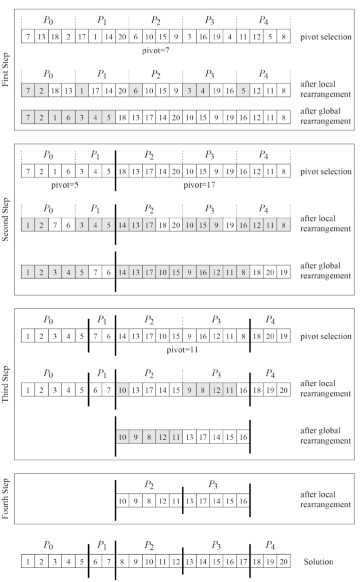
\includegraphics[scale = 2.0]{img/parallel quicksort.jpg}
        \label{quicksort par}
        \caption{Parallel QuickSort algorithm}
\end{figure}

This method suffers from the following \textbf{disadvantages}:

\begin{itemize}
    \item It requires a very high \textbf{parallelism degree};
    \item The \textbf{load balance} is still sensitive to the pivot selection.
\end{itemize}

\subsubsection{Odd-Even transposition}
This method works as follows:

\begin{enumerate}
    \item Repeat $\frac{n}{2}$ times:

    \begin{enumerate}
        \item Compare-exchange the \textbf{odd} elements with their immediate neighbor;
        \item Compare-exchange the \textbf{even} elements with their immediate neighbor.
    \end{enumerate}
\end{enumerate}

\begin{figure}[h!]
		\centering
		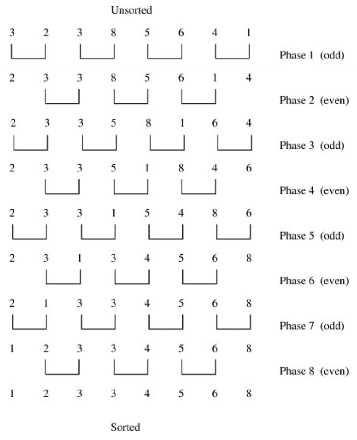
\includegraphics[scale = 2.0]{img/odd-even transposition.jpg}
        \label{odd-even}
        \caption{Odd-even transposition}
\end{figure}

Clearly, the \textbf{sequential} complexity is $O(n^2)$, so it is a bad sequential algorithm. On the other hand, each phase can be easily \textbf{parallelized}, and if the number of processors $p = \frac{n}{2}$, then each phase (compare odd or compare even) takes $O(1)$, so in total $O(n)$, so the overall complexity is $\frac{n}{2} * n = O(n^2)$. Since the complexity of sorting is $O(n \log n)$, this algorithm is not cost optimal.

However, this algorithm can be generalized by assigning batches of $n/p$ elements to each processor. In this case, the local sort on $n/p$ elements (i.e. the sort of each batch) takes $p (n/p \log (n/p)) = O(n \log (n/p))$, so in order to produce the result we need a linear scan of all the batches for each phase, so the cost is $p (p * n/p) = O(np)$. If $p = O(\log n)$, then the parallel algorithm is cost optimal with cost $O(n \log n)$. However, this strategy has the drawback that when increasing $p$, we must exponentially increase $n$ in order to have the same scalability, otherwise the algorithm would not be cost optimal anymore.

\subsection{Bitonic sort}
We now focus on another type of sort, and we will discuss a sequential algorithm which is not optimal, but easily to be parallelized (with an high parallel degree too).

A sequence $X = x_1, x_2, .., x_N$ is said to be \textbf{bitonic} if $x_1, .., x_j$ is \textbf{monotonically increasing} and $x_{j+1}, .., x_N$ is \textbf{monotonically decreasing}, or this holds for a cyclic shift of the input sequence.

\begin{figure}[h!]
		\centering
		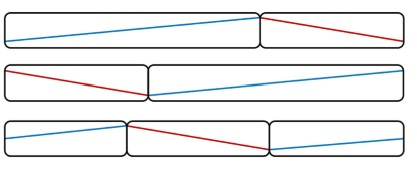
\includegraphics[scale = 2.0]{img/bitonic sequence.jpg}
        \label{bitonic seq}
        \caption{Examples of bitonic sequences}
\end{figure}

We now address two problems:

\begin{enumerate}
    \item How to sort a bitonic sequence?;
    \item Supposing that we can sort a bitonic sequence, how can we make a sequence bitonic?
\end{enumerate}

\subsubsection{Bitonic sort}
A \textbf{comparator} $[i:j]$ sorts the i-th and the j-th element of a sequence into a non-decreasing order. A \textbf{Bitonic split} is the result of applying N/2 comparators of the kind $[i:i + N/2]$ for $1 \leq i \leq N/2$ to a \textbf{bitonic sequence}. Picture \ref{bitonic split} shows the functioning of a bitonic split.

\begin{figure}[h!]
		\centering
		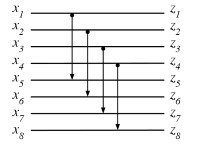
\includegraphics[scale = 2.0]{img/bitonic split.jpg}
        \label{bitonic split}
        \caption{Functioning of a bitonic split}
\end{figure}

The Bitonic split ensures two properties:

\begin{itemize}
    \item All the elements of the first half are less or equal the elements of the second half: if $Z = BS(X)$, i.e. $Z$ is the result of the Bitonic split of the input $X$, then:

    $$
    Z_1, .., Z_{N/2} \leq Z_{N/2 + 1}, .., Z_N
    $$

    \item Each of the halves is a bitonic sequence, i.e. $Z_1, .., Z_{N/2}$ and $Z_{N/2 + 1}, .., Z_N$ are bitonic.
\end{itemize}

Both the properties hold since the input sequence is bitonic.

Now, the idea of the algorithm is to \textbf{recursively} apply a \textbf{Bitonic split} to \textbf{each of the sequences}. Thus, a \textbf{Bitonic merge} performs recursive Bitonic splits until the resulting sequence is sorted in increasing order.

\begin{figure}[h!]
		\centering
		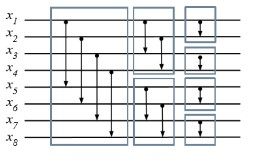
\includegraphics[scale = 2.0]{img/bitonic merge.jpg}
        \label{bitonic merge}
        \caption{Functioning of a bitonic merge}
\end{figure}

This method involves $\log N$ steps (where $N$ is the length of the input sequence), and each step performs $N/2$ compare/swap operations (i.e. bitonic splits). Thus, the \textbf{complexity of the sequential algorithm} is $O(N \log N)$.

If we have $N/2$ processors, than each comparison can be executed in parallel, so the \textbf{complexity of the parallel algorithm} is $O(\log N)$.

Before focusing on how we can make a sequence bitonic, we now discuss an interesting \textbf{property} of this algorithm. Indeed, in this method the \textbf{operations do not depend on the input data}, so the algorithm works for every input, provided that it is bitonic. Notice that this is a very good advantage, since it makes the algorithm easily parallelizable, exploiting an high parallelism degree. Notice also that this property does not hold for every algorithm, e.g. the operations of the QuickSort algorithm depend on the choice of the pivot.

\subsubsection{Constructing a Bitonic sequence}
In order to feed the final Bitonic Merge step with a bitonic sequence, the two halves of the input are sorted ascendingly/descendingly by recursively invoking Bitonic sort. 

\begin{figure}[h!]
		\centering
		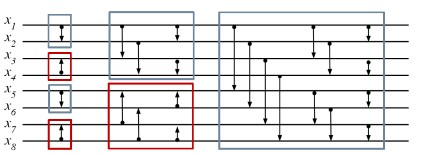
\includegraphics[scale = 2.0]{img/bitonic sort.jpg}
        \label{bitonic sort}
        \caption{Functioning of a bitonic merge}
\end{figure}

As we can see, there are $\log N$ Bitonic merge phases, each having complexity $N \log N$, so the overall complexity id $O(N \log^2 N)$. Notice that the Bitonic sort can be parallelized very well, and it can exploit a large parallelism degree. The parallel cost is $O(p \log^2 N)$, so it is not cost optimal, and this algorithm is very popular for GPUs and for medium sized inputs.
